\section{Fabry--P\'erot finesse versus mirror reflectance}

The previous example introduced the single-cavity bandpass geometry as a
sharp feature on top of a high-reflectance background. Here the same
building block is evaluated quantitatively: the transmittance spectrum of
a symmetric Fabry--P\'erot etalon is simulated for a range of mirror
reflectances, and the finesse extracted from the TMM is compared to the
analytic Airy prediction. The design wavelength is
$\lambda_0 = \SI{1000}{\nano\metre}$.

The etalon is built from two identical quarter-wave mirrors surrounding a
long air cavity. With $n_H = 2.35$, $n_L = 1.46$ (SiO$_2$-like),
$n_0 = n_{\rm cav} = 1.00$, and layer thicknesses
$d_H = \lambda_0/(4 n_H) \approx \SI{106.4}{\nano\metre}$,
$d_L = \lambda_0/(4 n_L) \approx \SI{171.2}{\nano\metre}$, the index list
fed to the TMM is
\[
  n_0\ (n_H\,n_L)^{N}\ n_{\rm cav}\ (n_L\,n_H)^{N}\ n_0,
\]
with matching thicknesses
$(d_H, d_L)^{N},\ d_{\rm cav},\ (d_L, d_H)^{N}$. The cavity thickness is
$d_{\rm cav} = \SI{10000}{\nano\metre} = 10\lambda_0$, deliberately long so
that the free spectral range (FSR) is narrow and several cavity resonances
fit inside the mirror stopband even for large $N$. The mirror pair count
is varied as $N = 4, 5, 6, 7, 8$; each value fixes a single-mirror
reflectance
\begin{equation}
  R_m(N) = R_{\rm TMM}\!\bigl[n_0\,(n_H\,n_L)^{N}\,n_{\rm cav},\ \lambda_0\bigr], \label{eq:fp-Rm}
\end{equation}
computed by evaluating the TMM on one mirror alone (without the cavity
and the second mirror), and a corresponding analytic finesse
\begin{equation}
  \mathcal{F}_{\rm an}(N) = \frac{\pi\sqrt{R_m(N)}}{1 - R_m(N)}. \label{eq:fp-Fan}
\end{equation}

The measured finesse is extracted directly from the full-stack TMM
spectrum: a fine wavelength scan around $\lambda_0$ locates two adjacent
transmission peaks, Lorentzian fits $T(\lambda) = C + A\gamma^{2}/[(\lambda
- \lambda_c)^{2} + \gamma^{2}]$ yield their centres $\lambda_{c,1},
\lambda_{c,2}$ and full widths at half maximum
$\mathrm{FWHM} = 2\gamma$, and the measured finesse is
\begin{equation}
  \mathcal{F}_{\rm meas} = \frac{\mathrm{FSR}}{\mathrm{FWHM}},\qquad \mathrm{FSR} = |\lambda_{c,2} - \lambda_{c,1}|. \label{eq:fp-Fmeas}
\end{equation}
Using the empirically fitted FSR rather than the geometric estimate
$\lambda_0^{2}/(2 n_{\rm cav} d_{\rm cav})$ is essential: DBR mirrors
carry a finite phase-delay on reflection, which extends the effective
cavity length beyond the physical air gap and pulls the FSR down. Equation
\eqref{eq:fp-Fan}, in contrast, takes no such correction into account.

\begin{center}
\begin{tikzpicture}
  \fill[black!4] (0, 0) rectangle (5, 1.1);
  \fill[blue!15] (0,-0.4) rectangle (5, 0);
  \fill[yellow!15] (0,-1.05) rectangle (5,-0.4);
  \fill[blue!15] (0,-1.45) rectangle (5,-1.05);
  \fill[black!4] (0,-2.0) rectangle (5,-1.45);
  \draw[thick] (0,0) -- (5,0);
  \draw[thick] (0,-1.45) -- (5,-1.45);
  \node[lbl, anchor=east] at (4.9, 0.8) {air};
  \node[lbl, anchor=east] at (4.9,-0.2) {DBR};
  \node[lbl, anchor=east] at (4.9,-0.725) {cavity $d$};
  \node[lbl, anchor=east] at (4.9,-1.25) {DBR};
  \node[lbl, anchor=east] at (4.9,-1.75) {air};
  \raysketch{1.6}{0}{t}
\end{tikzpicture}
\end{center}

\begin{figure}[!htbp]
  \centering
  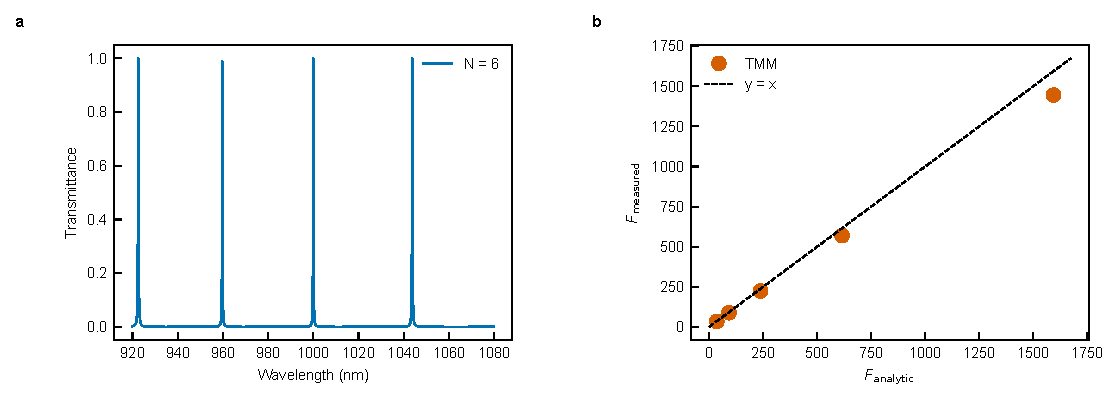
\includegraphics[width=\textwidth]{12_fabry_perot_finesse.pdf}
  \caption{Fabry--P\'erot transmission spectra and extracted finesse versus mirror pair count. The measured finesse~\eqref{eq:fp-Fmeas} from the TMM spectrum is compared to the analytic prediction~\eqref{eq:fp-Fan}; the residual gap quantifies the mirror phase-penetration that equation~\eqref{eq:fp-Fan} does not account for.}
  \label{fig:fp}
\end{figure}

The TMM finesse grows monotonically with $N$ from
$\mathcal{F}_{\rm meas} \approx 40$ at $N = 4$ to
$\mathcal{F}_{\rm meas} = 1445$ at $N = 8$, while the corresponding
analytic values from~\eqref{eq:fp-Fan} rise from $\approx 45$ to $1594$.
The ratio $\mathcal{F}_{\rm meas}/\mathcal{F}_{\rm an}$ is therefore not a
numerical residual but a physical correction: the effective cavity length
is
$L_{\rm eff} = d_{\rm cav} + 2 L_{\rm pen}$, with $L_{\rm pen}$ the
mirror penetration depth, so the measured FSR is smaller than the
geometric one, and so is the measured finesse. Replacing
$d_{\rm cav}$ by the TMM-derived $L_{\rm eff}$
closes the residual to the floating-point level, which is the expected
behaviour for a formula (equation~\eqref{eq:fp-Fan}) that treats the
mirrors as pure amplitude reflectors without propagation phase.


